\documentclass[../main.tex]{subfiles}
\graphicspath{{\subfix{../src/}}}

\begin{document}

%\subsubsection{Machine-Learning Designs}

%TODO: Some introduction and explanation of feature extraction, what types and papers that uses these.
%TODO: Some introduction and explanation of SVM and LDA types of networks.
%TODO: Go back and see what papers uses these.

%\subsection{Software Hand Design}

%\section{Tests \& Results}

\section{Datasets}
\subsection{Created Dataset}

As explained in section \ref{sec:motiveproblems}, creation of a custom dataset to train and test models on proved to be difficult.
The dataset created using the Motive Capture Software in section \ref{sec:motiveglove} during the development of this thesis is not very large, and has no labeling for classification.
Because of this, the dataset is not suitable for training in any of the methods.

\begin{figure}[H]
\begin{center}
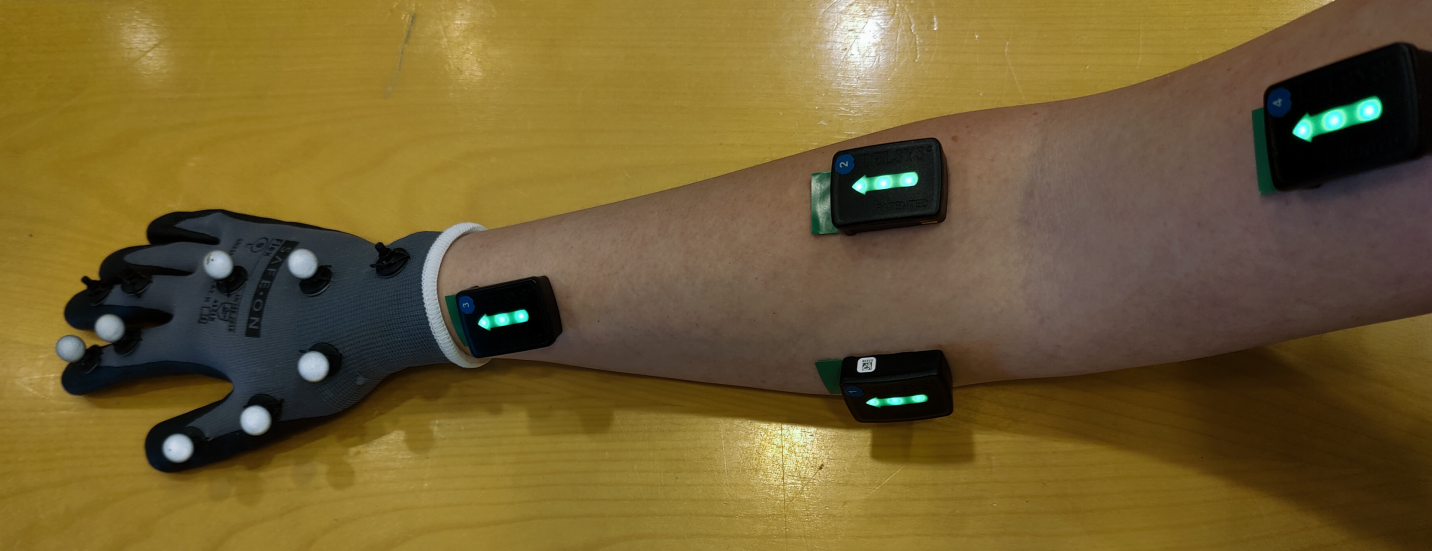
\includegraphics[width=0.99\textwidth]{sensors_on_arms_cropped.png}
\caption{Capture glove and sEMG sensors placed on the recording target. The sEMG sensors are located based on the muscles from table \ref{tab:muscletargets}.}
\label{fig:musclesensors}
\end{center}
\end{figure}

\subsection{Implementation}

Based on the literature review in Section \ref{sec:literature}, it becomes apparent that there exists a standard pipeline for translating sEMG recordings into predicted motor control for a prosthetic.
Raw sEMG data contains a lot of unwanted noise as explained in section \ref{sec:noise}.
Some of the noise can be can be removed through signal processing using analog filters.
Different filter types exists, and different filters are used to remove a specific frequency in the data. 
State-of-the-Art papers use a lot of different methods to reduce noise in sEMG data.
The paper \cite{multdof} proposes the use of a $50Hz$ Notch filter, while papers \cite{graspintent} \& \cite{ashirbad2022} respectively chooses a $20Hz$ cutoff Buttersworth filter \& a $10-500Hz$  Buttersworth band-pass filter, lastly the paper proposes a $60Hz$ notch filter in order to remove power-line noise.
Due to me many different filtering types used in state-of-the-art literature, it was determined that the use of a filter depends on the specific sEMG data and the purpose of what the paper tries to do.
In order to determine what types of filters have a positive effect on the sEMG data recorded using the Motive Capture system, different types of state-of-the-art pre-processing filters were tested and compared.
%And that the best filter for this thesis is to be determined through testing.

%TODO: Convert n sEMG angles into a image heat map kinda, and compare before and after different filters? the z dimension could be change in values?

\subsection{Tests \& Results}

A subset of the recorded sEMG data was used, and different filter types were tested in order to reduce noise in the raw recordings.
Different types of Buttersworth filters were tested, as can be seen in figure \ref{fig:lowpass} \& \ref{fig:bandpass}.

\begin{figure}[H]
\begin{center}
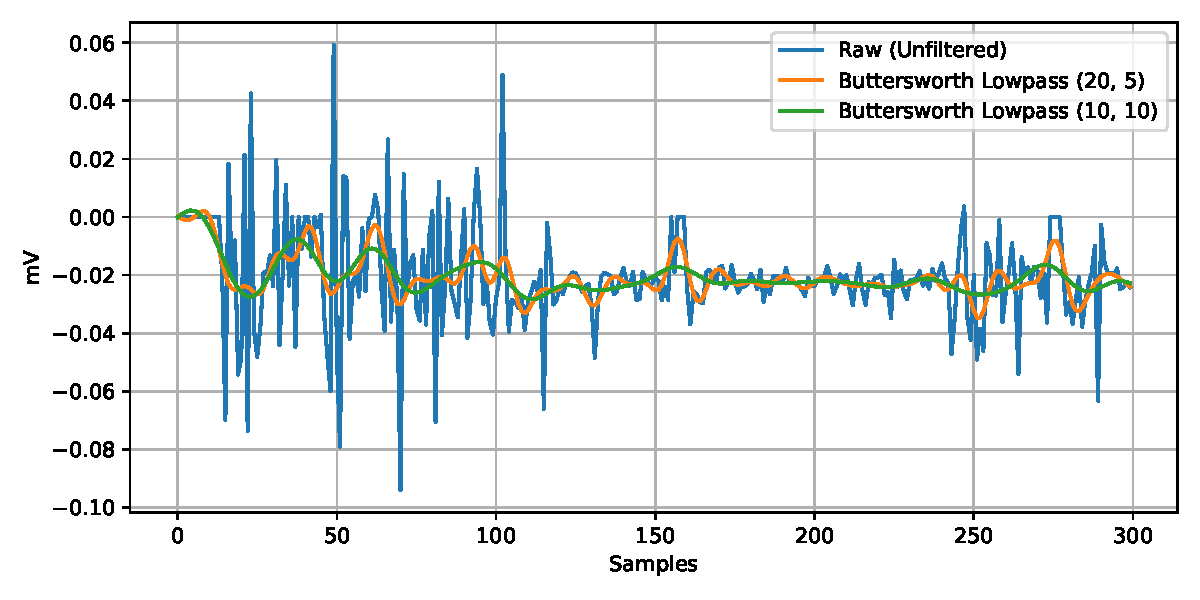
\includegraphics[width=0.99\textwidth]{lowpass.pdf}
\caption{Comparison of Buttersworth low-pass filters of different cutoff frequencies and orders.}
\label{fig:lowpass}
\end{center}
\end{figure}
\begin{figure}[H]
\begin{center}
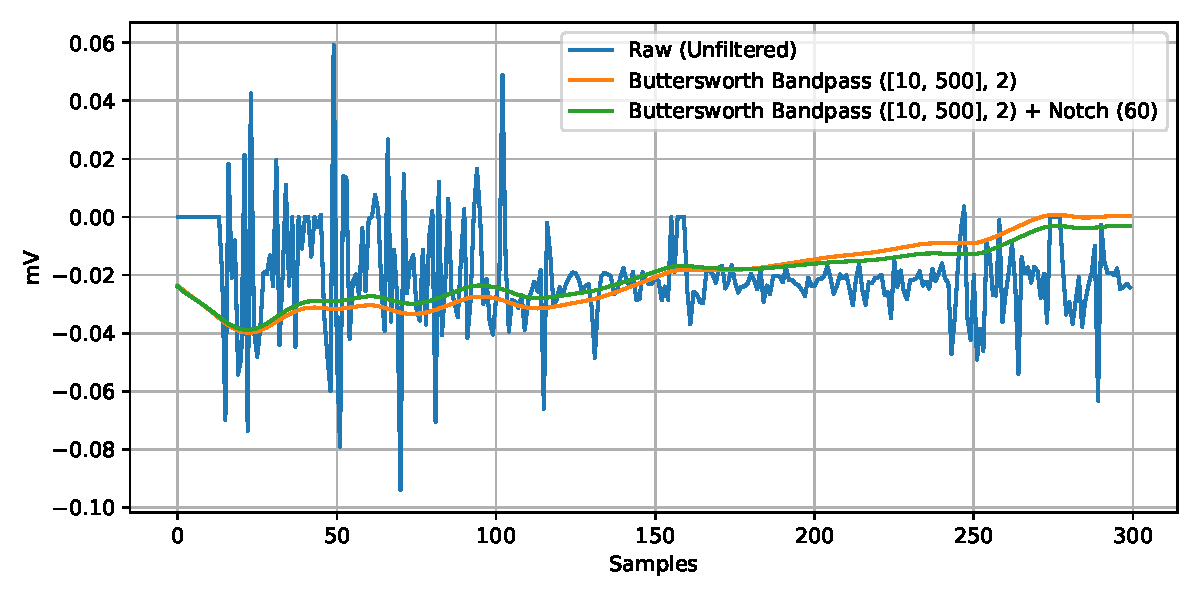
\includegraphics[width=0.99\textwidth]{bandpass.pdf}
\caption{Comparison of Buttersworth band-pass filters of different cutoff frequencies, orders and the usage of a Notch filter.}
\label{fig:bandpass}
\end{center}
\end{figure}

\subsection{Evaluation}

As can be seen in the figure, different configurations of pre-processing filters have a large impact on the resulting filtered sequence. 
It can be seen in figure \ref{fig:lowpass} that most of the change in amplitude exists in the low frequencies, and these are removed due to using a low-pass filter.
Furthermore, it can be seen that the intent of the signal is kept when a filter order of 5 is used, compared to a filter order of 10.
When comparing the two low-pass filters, it can be determined that using a cutoff frequency of $20Hz$ and a order of $5$ is a ideal for sEMG signals due to the amount of large frequencies in the recordings.
Alternatively, Buttersworth band-pass filters are tested in figure \ref{fig:bandpass},


\subsection{Dataset used for Training}

Due to the problems with the Motive motion capture software explained in section \ref{sec:motiveproblems}, it was determined that the main dataset for training the chosen methods would be based on dataset \cite{kinmusdataset} from the paper \cite{jarque2019}.
The dataset contains sections of sEMG data and kinematic movements of the hand.
These sections are labeled as either \textit{reaching}, \textit{manipulation} or \textit{releasing}.  
Due to the dataset containing data for regression and classification, it is possible to explore multiple methods of HMI's. 
The pre-processing step is not covered for the training dataset \cite{kinmusdataset}, as the dataset has been pre-processed using a 4th-order band-pass filter with a band of  $25$ to $500Hz$, then the data was subject to a 4th-order low-pass filter at $8 Hz$.
The main objective of these tests are to review and compare possible methods of regression \& Classification of sEMG data in order to determine the movements of the hand.

\newpage
\section{Machine-Learning Intent Classification}
\label{sec:machine-learning}

Due to the dataset containing labels associated with movements of the hand, it is possible to use the dataset to train a intent prediction classifier.
As mentioned in the papers \cite{Batzianoulis2018} \& \cite{Yuki2023}, it is ideal to feature extract windows of the raw sEMG data.
The papers propose that the features \textit{Zero Crossing} \& \textit{Root Mean Square} are ideal for intent classifiers.
Furthermore, the paper \cite{YanchaoWang2022} proposes that the Machine-Learning classifier LDA has the highest classification rate out of similar methods.
The paper \cite{Batzianoulis2018} proposes the use of the \gls{SVM} \gls{ML} method for intent classification.
Both types of classification will be explored and compared.

\subsection{Implementation}

In order to classify intent from sEMG muscle data, the data needs to be converted to feature space before it can be used as input to a machine learning algorithm.
For this, it was chosen based on state-of-the-art literature, that the feature extraction methods would be zero-crossing \& RMS.
The input channel for a single sEMG window was converted into a vector of zeros and ones for the zero-crossing features, where a one is set if the data crosses over the zero line.
Furthermore, the RMS for a window was calculated, and inserted to the end of the input vector. This effectively converts the 6 sEMG channels of a window size of $N$ into a feature vector of size $N+1$.
The feature-based inputs were extracted, and their movement labels were used as the target classification.

\begin{figure}[H]
\begin{center}
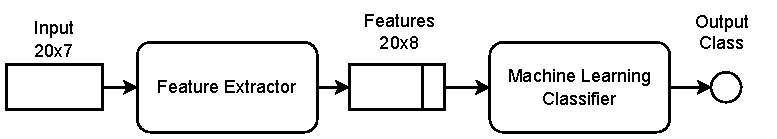
\includegraphics[width=0.99\textwidth]{MLClassifier.pdf}
\caption{The machine learning classifier setup with a feature extraction step.}
\label{fig:mlclassifier}
\end{center}
\end{figure}

The dataset of features and ground truths were then used as input for discriminant analysis, and SVM classifiers.
The purpose of \textbf{discriminant analysis} is to classify inputs into groups.
Discriminant analysis is a classical multivariate method of Supervised Learning, that takes a input set with their ground-truth classes and tries to maximize separation between these different classes.
The models assumes that data follows a Gaussian distribution. 
%TODO: True? Cite something for LDA QDA?
For this ML method, two types of discriminant analysis were tested on the dataset, namely \gls{LDA} \& \gls{QDA}.
%Linear Discriminant Analysis (LDA) \& Quadratic Discriminant Analysis (QDA).
The main difference between LDA and QDA is that LDA makes the assumption that the covariance matrices of the classes are the same.
Equal covariance matrices will result in linear separations between classes.
QDA as an alternative does not assume this equal covariance, this results in a classifier that assumes quadratic separations between classes.
%The first method to test is the Linear Discriminant Analysis (LDA), and the second method was 
Just as discriminant analysis, SVM based methods are used to separate inputs into groups based on classes.
SVM is a robust supervised learning method that groups dataset classes.
SVM tries to maximize the width between classes by converting the input to a higher dimensional feature vector, and using this vector, the SVM algorithm is able to efficiently calculate a non-linear classification.
The feature space conversion is determined by the choice of SVM kernel in the algorithm.
For this ML method, 3 types of SVM classifiers were tested, a SVM using a Radial Basis Function (RBF) kernel, a SVM using a sigmoid Kernel and a NuSVM method with the RBF kernel and a parameter for the number of support vectors used.

\subsection{Tests \& Results}

The methods are tested on 50 sets of data that was not part of the training set.
The discriminant analysis methods can be seen in figure \ref{fig:lda_test}, with the average accuracy of the methods respectively being $0.61\%$ \& $0.55\%$ over the 50 tests.

\begin{figure}[H]
\begin{center}
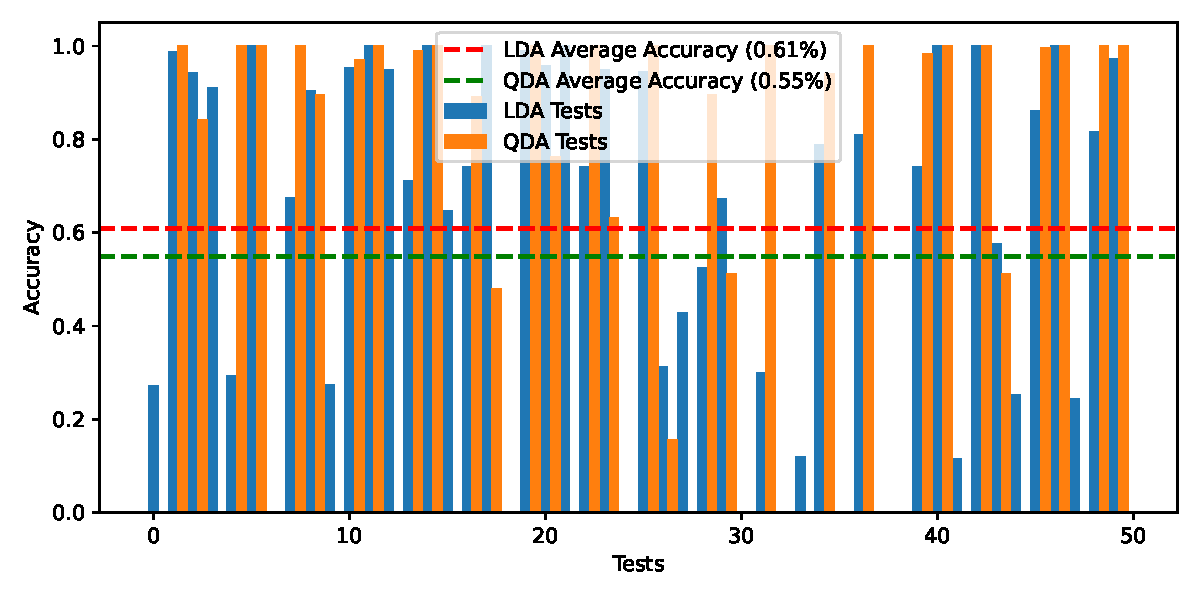
\includegraphics[width=0.99\textwidth]{lda_test.pdf}
\caption{Comparison of discriminant analysis methods (\gls{LDA}/\gls{QDA}) over 50 tests.}
\label{fig:lda_test}
\end{center}
\end{figure}
%TODO: Graphs does not show what bar is what type..

The \gls{SVM} methods can be seen in figure \ref{fig:svm_test}, with the average accuracy of the methods respectively being $0.54\%$, $0.56\%$ \& $0.59\%$ over the 50 tests.

\begin{figure}[H]
    \centering
    \begin{subfigure}[b]{1\textwidth}
        \centering
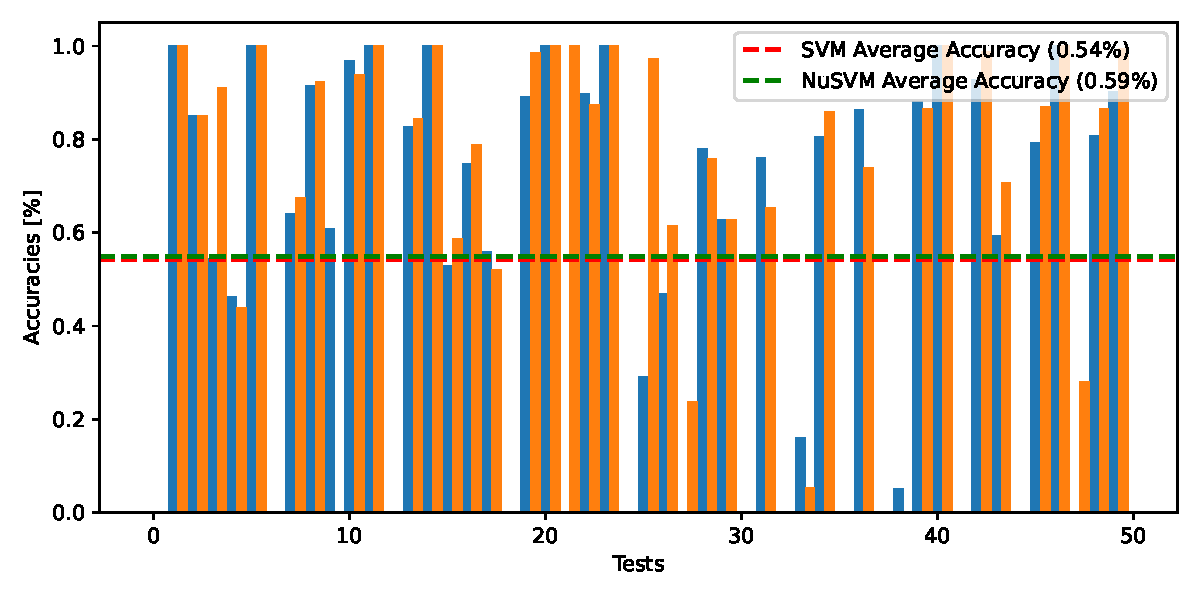
\includegraphics[width=0.99\textwidth]{svm_test.pdf}
%\caption{Comparison of Support Vector Machine Kernels (RBF/Sigmoid) over 50 tests.}
    \end{subfigure}
    \centering
    \begin{subfigure}[b]{1\textwidth}
        \centering
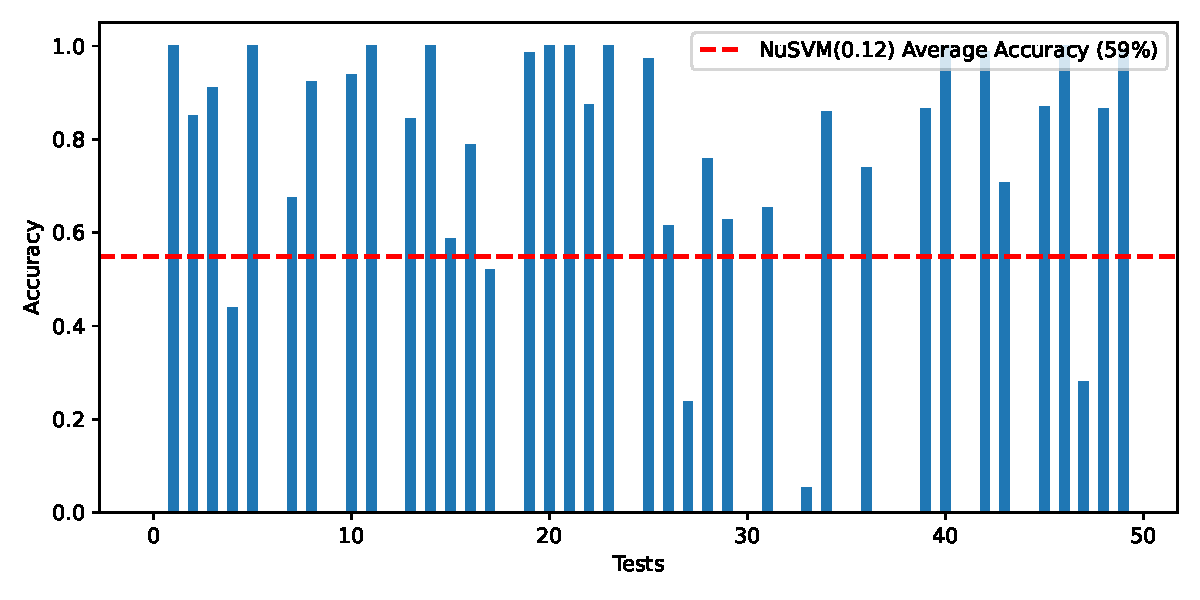
\includegraphics[width=0.99\textwidth]{nusvm_test.pdf}
    \end{subfigure}
    \caption{Comparison of \gls{SVM} Kernels \& parameters over 50 tests.}
\label{fig:svm_test}
\end{figure}
%TODO: Try another parameter for NuSVM so that the graph is more complete.

\subsection{Evaluation}

%TODO: GO through the graphs and talk about the results
The methods tested can be seen to have similar average accuracy of $\sim 0.6\%$ over 50 tests.
Because of this, it is difficult to choose a superior method without further analysis.
The choice of machine learning method depends on its overall classification rate over 50 tests, but it can also be important to rate the ML methods based on their inter-quantile values.
A full comparison of the machine learning methods can be seen in figure \ref{fig:classification_comparison}.

\begin{figure}[H]
\begin{center}
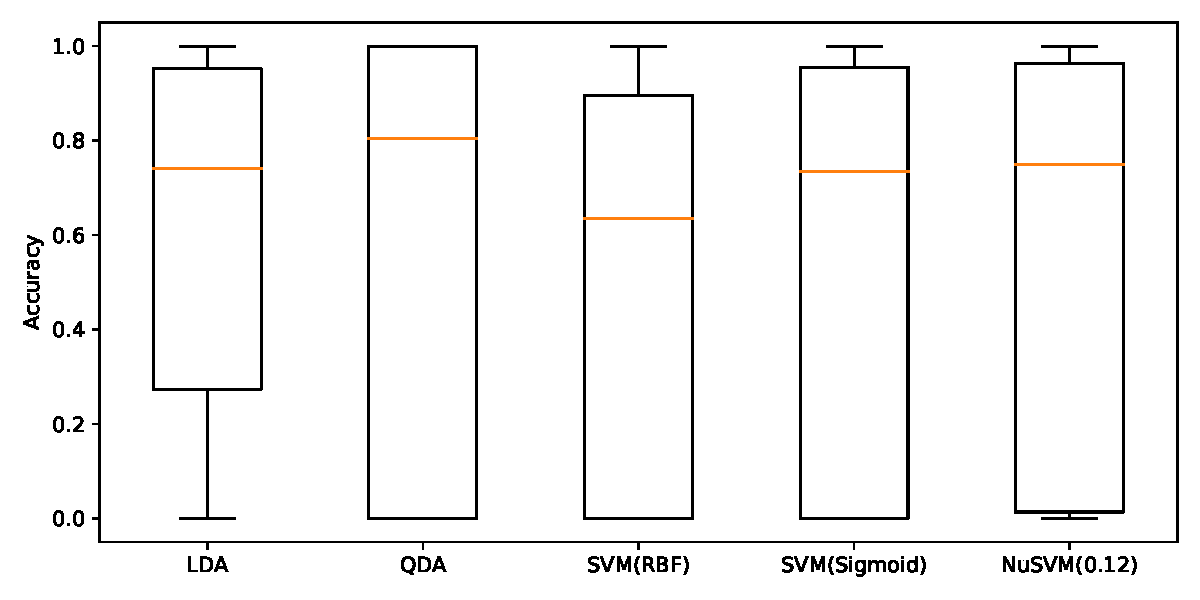
\includegraphics[width=0.99\textwidth]{classification_comparison.pdf}
\caption{Comparison of chosen classification methods based on accuracy over 50 tests.}
\label{fig:classification_comparison}
\end{center}
\end{figure}

It can be seen in the boxplot that most methods have a similar inter-quantile median, and fairly small whiskers.
In order to get a clearer comparison of methods, the relevant values have been compared in table \ref{tab:classification_comparison}.  

\begin{table}[H]
\begin{center}
\begin{tabular}{ |l|c|c|c| } 
 \hline
 ML Method & avg-accuracy [\%] & Inter-quantile Median & Inter-quantile Range \\ 
 \hline
 LDA & \textbf{0.61\%}           & 0.741705 & \textbf{0.679410} \\ 
 QDA & 0.55\%           & \textbf{0.803432} & 1.000000 \\ 
 SVM (RBF) & 0.54\%     & 0.634426 & 0.895688 \\ 
 SVM (Sigmoid) & 0.56\% & 0.735050 & 0.955580 \\ 
 NuSVM (0.12) & 0.59\%  & 0.749436 & 0.950715 \\ 
 \hline
\end{tabular}
\caption{Comparison of relevant classification parameters for the chosen methods. The best performing parameters have been highlighted.}
\label{tab:classification_comparison}
\end{center}
\end{table}
%         label  lower_whisker  lower_quartile    median  upper_quartile  upper_whisker
% 0          LDA             0.0        0.273173  0.741705        0.952582            1.0
% 1          QDA             0.0        0.000000  0.803432        1.000000            1.0
% 2      SVM(RBF)            0.0        0.000000  0.634426        0.895688            1.0
% 3  SVM(Sigmoid)            0.0        0.000000  0.735050        0.955580            1.0
% 4   NuSVM(0.12)            0.0        0.013333  0.749436        0.964048            1.0

% Inter-Quantile range
% 0    0.679410
% 1    1.000000
% 2    0.895688
% 3    0.955580
% 4    0.950715

The relevant parameters in the table makes it possible to identify the most suitable method for intent classification.
It can be seen that LDA has the overall best accuracy of all the methods of $61\%$, and the overall worst performing method is SVM (RBF).
By denoting the median and the range of the inter-quantile section of the boxplots, we can further elaborate on the accuracy of the 50 tests.
% LDA
LDA has the best average accuracy, and it also has the smallest inter-quantile range, indicating that LDA perform well across tests with a robustness to outlier tests. 
% QDA
It can be seen that QDA performs best according to the inter-quantile median, but QDA is also the method that has the largest inter-quantile range indicating that QDA is not very robust to outlier tests.
% NuSVM
An alternative to the discriminant analysis methods, it can be seen that the NuSVM method with a number of support vectors denoted by $0.12$.
NuSVM has the second best average accuracy, the second best inter-quantile median \& the third lowest inter-quantile range.
% Conclusion:
From the table \ref{tab:classification_comparison}, it becomes apparent that none of the methods have ideal performance, but that the LDA method is the best method for intent classification.
This result is similar to the conclusion in paper \cite{KeunTaeKim2021}.
% Eval on feature extraction
The resulting performance metrics of the ML methods are dependent on the chosen feature extraction techniques used.
Zero crossing and MSE features can be used for the classifiers and provide insight into what parameters are important when working with sEMG data.

\newpage
\section{Neural Network Movement Regression}
\label{sec:regression}

\subsection{Windowed Convolutional Neural Network}

As an alternative to intent classification, the dataset could be used to train finger movement regression networks.

\subsubsection{Implementation}

%TODO: WHY CHOOSE A CNN? SELL IT LIKE A CAR!
The sEMG data used as input for regression networks is complex.
The sequences of muscle activity needs to be understood by the proposed method and produced into a an output.
A network type that is ideal to understand complex meaning in, 3-dimensionary inputs is a CNN network.
%A CNN is an alternative to a MLP network that is similar in functionality is a Convoluted Neural Network (CNN).
A CNN consists of a set of Convolution Layers that deforms inputs to abstract convolution features.
The structure is considered sparsely connected due to the convolution layers are only receiving a subset of the previous convolution features.
The feature conversion is ideal when a network needs to become robust and needs to recognize larger concepts in the input.
This functionality is especially used when the input data takes the shape of a matrix.
Once the input is convoluted to a chosen feature abstraction, it is given to a MLP structure trained to convert the convolution features into a usable output.
%TODO: needs sources for this stuff?
%TODO: Go back and see what papers uses CNN's
CNN networks have no build-in time-based functionality, they receive a set of inputs and produce an output.
It is possible however to represent time if the input is given in segments consisting of multiple time-frames.
Because of this, the sEMG muscle activity from the dataset is segmented into windows of a desired size, the output angles that the network should do regression towards are then chosen to be the first angle after the window.
%TODO: Images of these for better clarity!!!!
A CNN network can be used in the field of sEMG processing due to the convolution layer's ability to learn abstract formations of the sEMG data.
The network would be able to identify patterns in sEMG data and correlate them to an appropriate output.
%TODO: formations? another word?
The CNN network structure seen in figure \ref{fig:cnn_structure}.

\begin{figure}[H]
\begin{center}
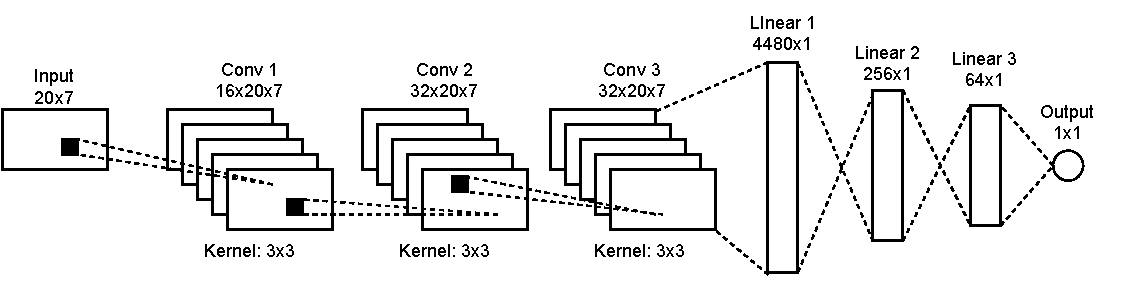
\includegraphics[width=0.99\textwidth]{cnnstructure.drawio.pdf}
\caption{The chosen CNN network structure, consisting of 3 Convolution Layers and 3 Linear layers. Network input is a window of sEMG recordings, with the purpose of regression of a finger joint angle.}
\label{fig:cnn_structure}
\end{center}
\end{figure}
%TODO: The 20 in this case refers to N samples! if i want something else than 20, change the image!

As visualized in the figure, the CNN network consists of 3 Convolution layers followed by 3 MLP layers.
The chosen CNN network structure is chosen to be simple due to the small input window of 7 muscle sensors and a window size of 20 samples.
For this reason, no pooling was used between the convolution layers.
The Convolution layers extract features up to a size of 32 using a convolution kernel with a size of [$3, 3$].
The convolution features are then flattened, to a size of $4480$, before being subject to the MLP layers that convert the extracted features into a regression prediction. 
%A CNN is trained on the network, using a window size of 40 samples were used.
%TODO: Give example of a state-of-the-art paper CNN as an alternative to mine!!!

The CNN network is trained to do regression of joint angles of the hand, because of this, the loss function is determined to be MSE loss.
The network is trained using an Adam optimizer with a learning rate of $1\text{e}^{-4}$.
A subset of the dataset is split into a test and a validation set, and windows are extracted correlating input and output.
The output is normalized, and the input/output sets are shuffled before training takes place.

\subsubsection{Tests \& Results}

In order to test the CNN network and assess its performance, the training MSE loss can be seen in figure \ref{fig:cnntrainvalid}.
%TODO: Make sure this graph is explained properly and is the actual image

\begin{figure}[H]
\begin{center}
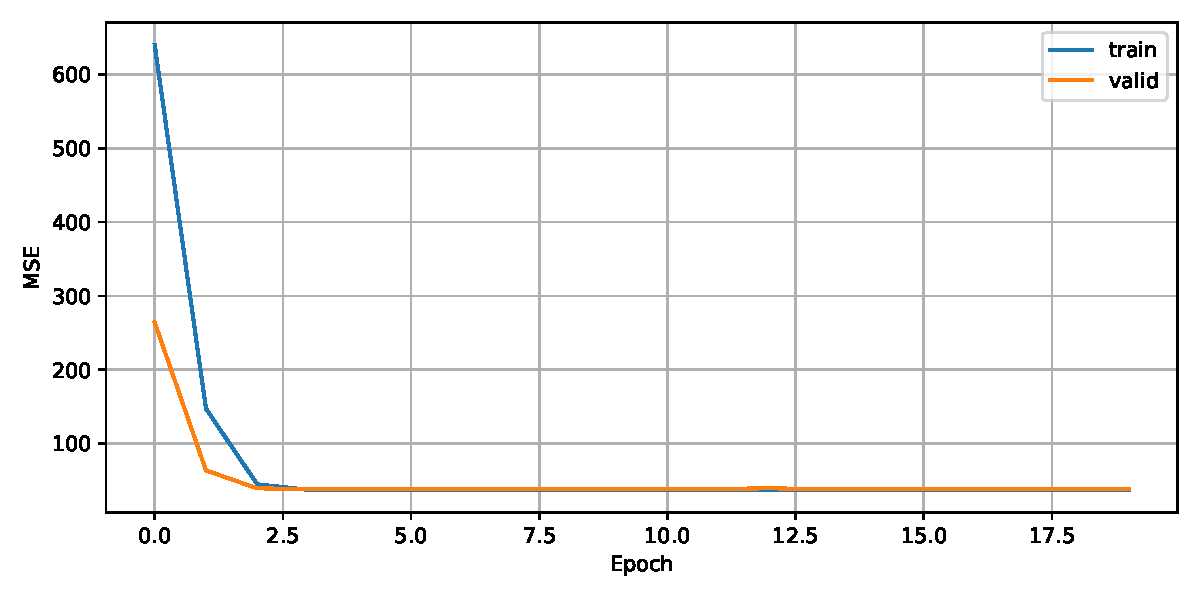
\includegraphics[width=0.8\textwidth]{cnn_trainvalid.pdf}
\caption{The Train and Validation MSE loss during training of the CNN network method.}
\label{fig:cnntrainvalid}
\end{center}
\end{figure}

The CNN network is trained with a batch size of 8 over 20 epochs, but as can be seen in the figure, the MSE loss settles at $\sim 34$ after just 3 epochs.

50 sets of regressions that have not been trained on are taken from the dataset for testing.
The errors of the dataset are plotted, as can be seen in figure \ref{fig:cnntest}.

\begin{figure}[H]
\begin{center}
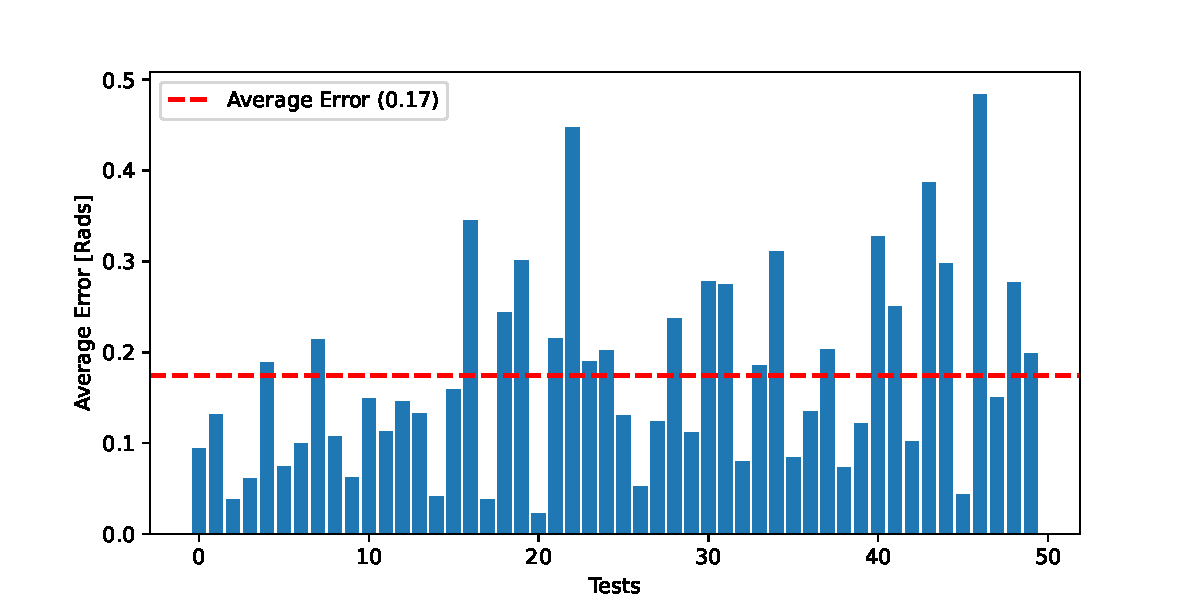
\includegraphics[width=0.99\textwidth]{cnn50test.pdf}
\caption{The errors of 50 regressions using the CNN network.}
\label{fig:cnntest}
\end{center}
\end{figure}
%TODO: What i need to do:
% Pull out 50 sets of data, do regression using my cnn model, plot their average errors in a barplot!
% This method will be my main regression test!


\subsubsection{Evaluation}

As can be seen in figure \ref{fig:cnntrainvalid}, the CNN network is able to be trained on the dataset with a validation set MSE loss of $0.34$.
The errors of the 50 test regressions in figure \ref{fig:cnntest} show that a fairly large average regression error of $0.17$ Radians exists in the test regressions, and that the average error is skewed upwards due to some outlier tests having large average errors up to $0.3$ Radians.
%TODO: Get the max error!

%TODO: Maybe do a average error boxplot too?


\subsection{Recurrent Neural Network Regression}

Due to sEMG data being time-based, Recurrent network types are ideal for regression predictions.
RNN networks are similar to MLP's with the main difference being that a RNN has hidden feedback  memory state that is derived from earlier inputs.
This functionality makes RNN networks ideal for concurrent, time-based systems where a sequential input distribution needs to be converted to a output regression.  
%TODO: Alternative to concurrent -> i want something that explains a set of data in a graph!
Another use case of RNN-based regression systems are systems where response time is critical.
The RNN network does not use a window of data, it converts the input of the current time frame, and the feedback of the previous time frame into a prediction.
Because of the hidden memory, a RNN network has a quicker response time than a window-based network.
The RNN network structure designed to predict regression of finger movements from sEMG data can be seen in figure \ref{fig:rnn_structure}.
%TODO: This one sounds nice, can it be integrated?
%The recurrent feedback loop correlates previous predictions with future predictions, allowing the network to approximate regressions per time frame.

\begin{figure}[H]
\begin{center}
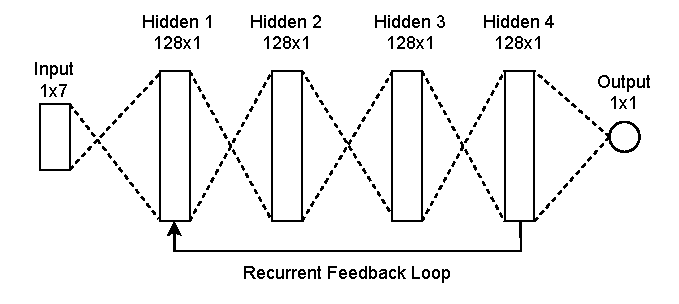
\includegraphics[width=0.8\textwidth]{rnnstructure.pdf}
\caption{The chosen RNN network structure, consisting of a input layer, 4 hidden layers with a recurrent feedback loop, and a output layer.}
\label{fig:rnn_structure}
\end{center}
\end{figure}

\subsubsection{Tests \& Results}

The RNN network is trained on the dataset \cite{kinmusdataset}, in a similar way as the CNN network, with the purpose of approximating finger angle regressions per time frame.
The RNN network is trained with a batch size of 8, with the  MSE loss function and the Adam optimizer with a learning rate of $1\text{e}^{-2}$.
In order to test the network, a random set of 50 regressions that have not been trained on are taken from the dataset.
The average errors of each regression test is plotted, as can be seen in figure \ref{fig:rnntest}.

\begin{figure}[H]
\begin{center}
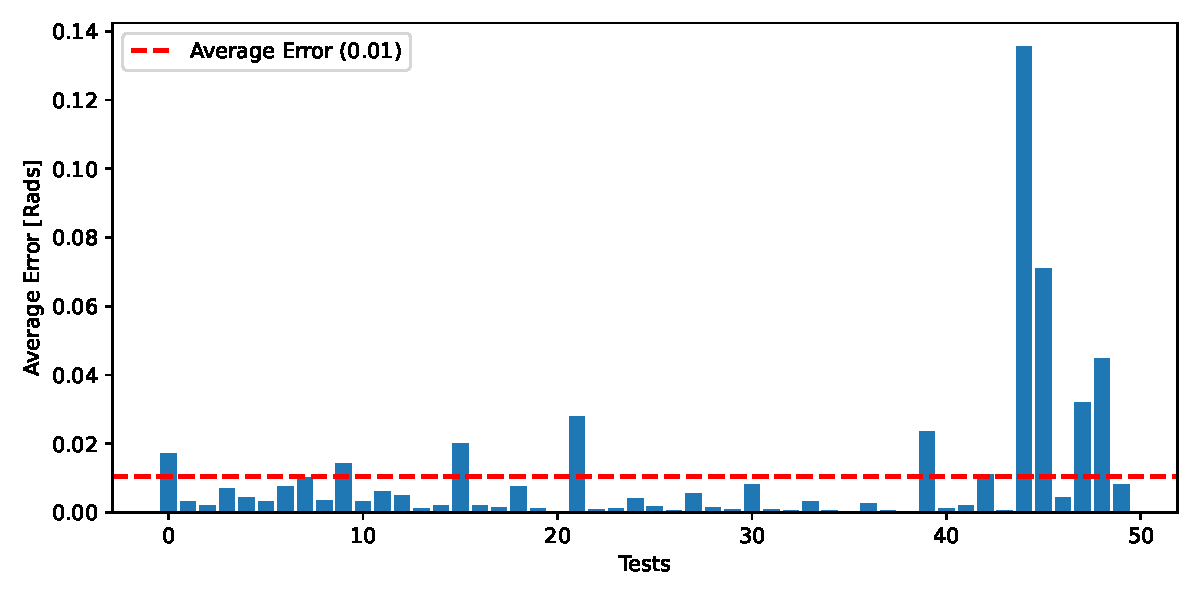
\includegraphics[width=0.99\textwidth]{rnn50test.pdf}
\caption{The errors of 50 regression tests using the RNN network.}
\label{fig:rnntest}
\end{center}
\end{figure}

\newpage
\subsection{Evaluation of Regression Methods}

%As can be seen in figure \ref{fig:cnntrainvalid}, the CNN network is able to be trained on the dataset with a fairly low MSE loss.  
The errors of the 50 test regressions in with the different models can be seen in figure \ref{fig:regression_comp}.

\begin{figure}[h]
\begin{center}
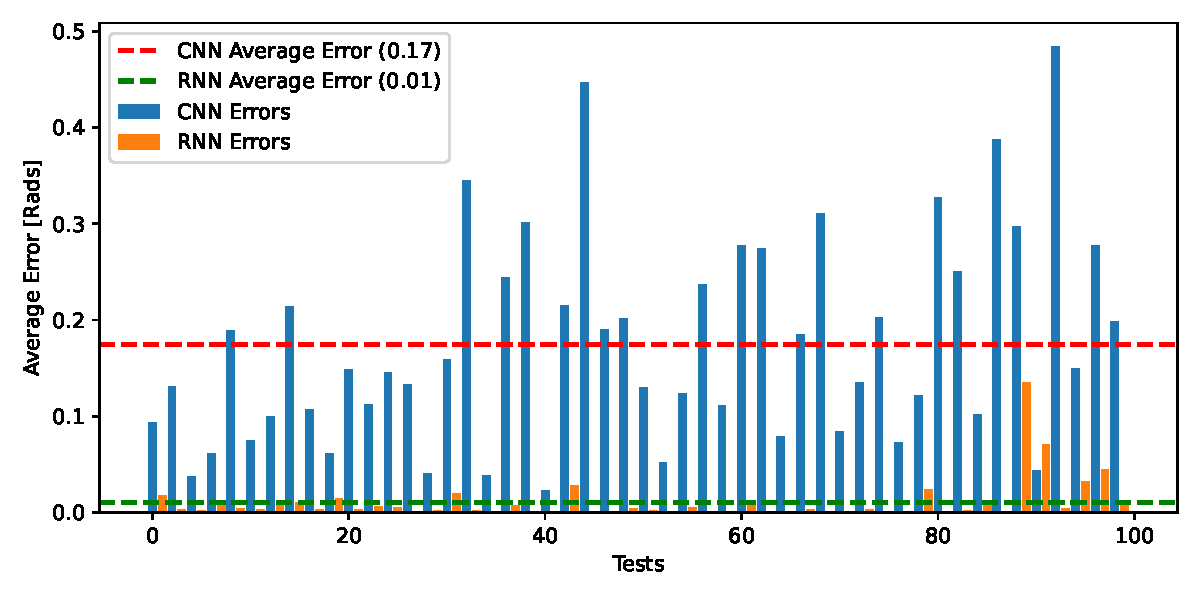
\includegraphics[width=0.99\textwidth]{regression_comparison.pdf}
\caption{Comparison of Windowed CNN and RNN regression methods.}
\label{fig:regression_comp}
\end{center}
\end{figure}

The figure clearly shows that there is a large difference in window-based and recurrent network types.
The CNN shows a average test error of $0.17$ Radians, while the RNN network has a average test error of $0.01$ Radians. 
The reason for the large error in the CNN network test is unclear.
One of the reasons the CNN network is unable to accurately learn regression could be because of the pre-processing done in the dataset.
Alternatively, the network is unable to learn because of the window size. This would make sense since the RNN network with a really low error is able to learn to do regression, as it is not limited by a arbitrary window of input.

It becomes apparent that teaching a neural network to do regression of finger joints is a complicated task.
Because of this, the tests propose that it is ideal to use a type of Recurrent Network for regression.

%TODO: Maybe do a average error boxplot too?

%TODO: Some introduction and explanation of RNN and LSTM types of networks.
%TODO: Go back and see what papers uses these.

%\subsubsection{Long-Short-Term-Memory Recurrent Neural Networks}
%TODO: Create this if you have the time..
%A variant of a RNN can contain a special kind of hidden memory called Long Short Term Memory (LSTM).
%a LSTM uses gates as a way of containing a memory.

%\section{Comparison of Regression-based Networks}

%\subsection{Feature-Based Multi Layer Perceptron Network}

%Neural Networks are widely used in the field of AI.
%One type of widely used neural network is a fully-connected Multi-Layer Perceptron (MLP) Network.
%The MLP network is popular due to its structure and training capabilities.
%A MLP consists of layers of weighted activation functions where each activation function in a layer recieves the entire previous layer's output summed up as input.
%Due to the structure of a MLP, the network is capable of recieving a set of inputs and be trained to approximate a n'th degree polynomial function that relates the given inputs and outputs.
%The network is trained by updating the individual weights through backpropagation with the predicted output and a ground-truth output.
%The MLP network could be used to predict the relation between muscle activity and finger movements.

%In order to initially test the the dataset, a simple MLP network will be trained as a baseline for performance, and for testing the general applicability of window-based networks.


%TODO: Explain the software i made to clearn motive!
%TODO: Explain and showcase some pre-processing filters mentioned by other papers!
%TODO: Maybe here, maybe in methodology: Show how the gt angles are calculated too..

\newpage
\section{Simulated Prosthetic Hand}
\label{sec:simtest}

\subsection{Useability of the Simulated Prosthetic Hand}
%\subsection{Anatomical Assessment and Maneuverability}

Access to existing prosthetic hand simulations proved to be impossible to access and use, as explained in section \ref{sec:hand_alternatives}. they are either unavailable because their associated products have been discontinued or locked behind a pay-to-access barrier where you have to pay to receive a real prosthetic.
Due to non-availability of prosthetic hand simulations, it was chosen that through this thesis, a open source prosthetic hand needed to be created for testing of the algorithms developed as part of this project.
The creation of a prosthetic hand simulation can be seen in section \ref{sec:prost_sim}.
The prosthetic hand was designed to be as anatomically similar as a real hand as possible.
This was done in order to accurately simulate the movement of a real hand, and because of it, allow users to test and validate control methods on a simulation before needing to construct a real prosthetic.
The usability and dynamic movement of the simulated prosthetic hand needs to be assessed.
This is important because the usability of a prosthetic hand has a large impact on rehabilitation for the end-user.

\subsection{Method}
In order to test the usability and dynamic movement of the simulated prosthetic hand, the hand was tasked with achieving the end-poses of the most used day-to-day grips.
These grips were explained in section \ref{sec:dataset} table \ref{tab:grips}, namely the \textit{Pulp pinch}, \textit{Lateral pinch}, \textit{Five-Finger pinch} \& \textit{Diagonal Volar grip (Power grip)}.
In order to pose the simulated hand, the interface created in ROS2 was used to send kinematic configurations to the hand simulation.

\subsection{Test \& Results}

The hand was posed into all 4 day-to-day grip configurations for visual assessment.
The resulting configurations of the hand can be seen in figure  \ref{fig:hand_pose_test}.
The software used to pose the hand simulation can be seen in appendix \ref{appendix:roscontrol} 

\begin{figure}
    \centering
    \begin{subfigure}[b]{0.49\textwidth}
        \centering
        %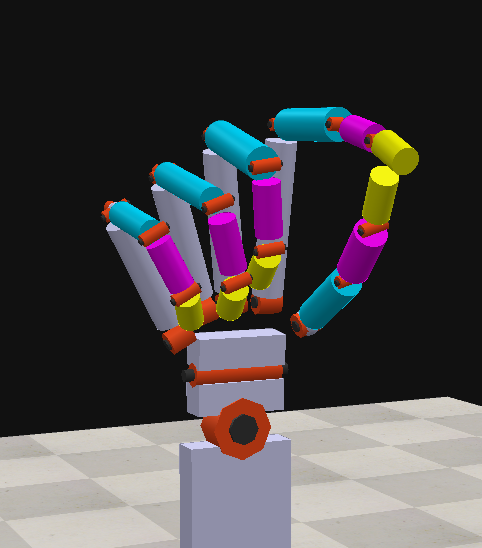
\includegraphics[width=\textwidth]{pulppinch_grip.png}
        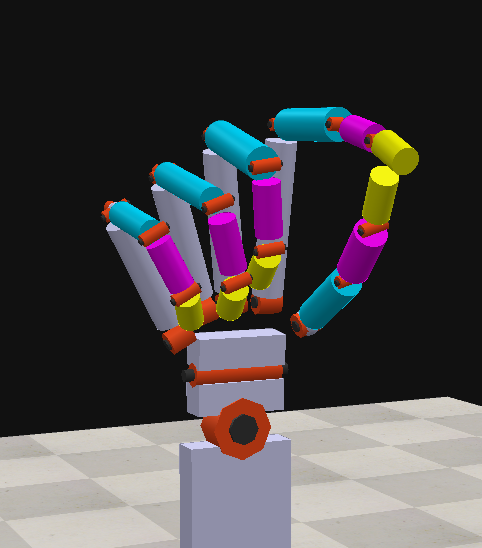
\includegraphics[height=8cm]{pulppinch_grip.png}
        \caption{Pulp pinch}
    \end{subfigure}
    \hfill
    \centering
    \begin{subfigure}[b]{0.49\textwidth}
        \centering
        %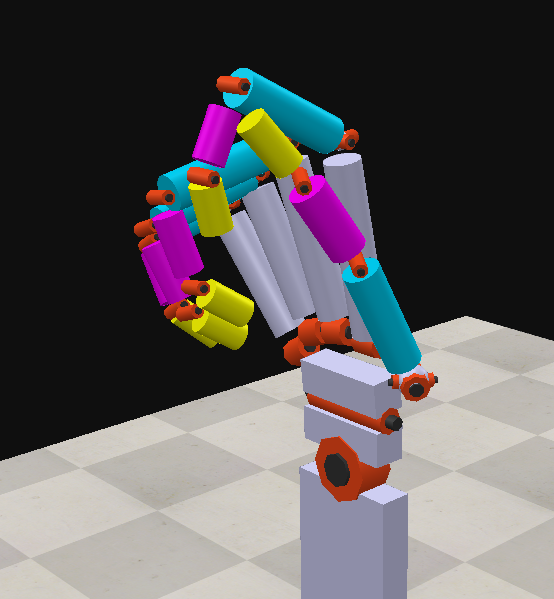
\includegraphics[width=\textwidth]{lateralpinch_grip.png}
        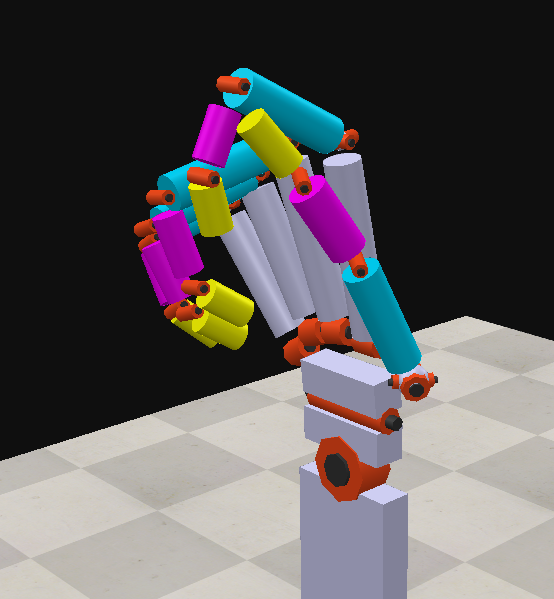
\includegraphics[height=8cm]{lateralpinch_grip.png}
        \caption{Lateral pinch}
    \end{subfigure}
    \hfill
    \begin{subfigure}[b]{0.49\textwidth}
        \centering
        %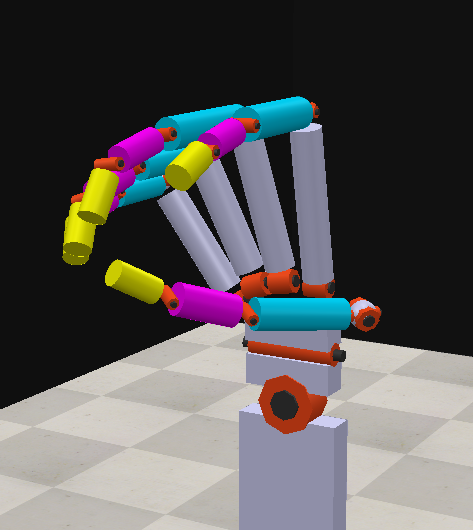
\includegraphics[width=\textwidth]{fivefingerpinch_grip.png}
        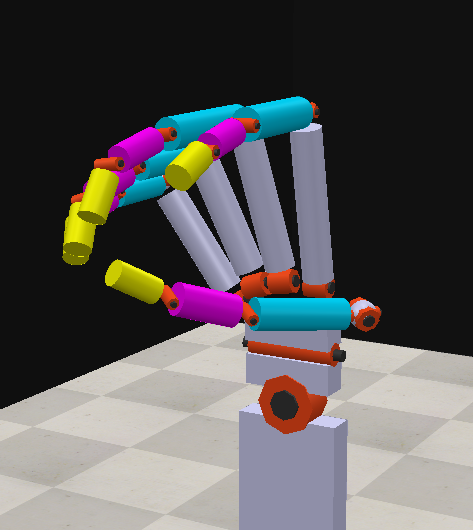
\includegraphics[height=8cm]{fivefingerpinch_grip.png}
        \caption{Five-Finger pinch}
    \end{subfigure}
    \hfill
    \begin{subfigure}[b]{0.49\textwidth}
        \centering
        %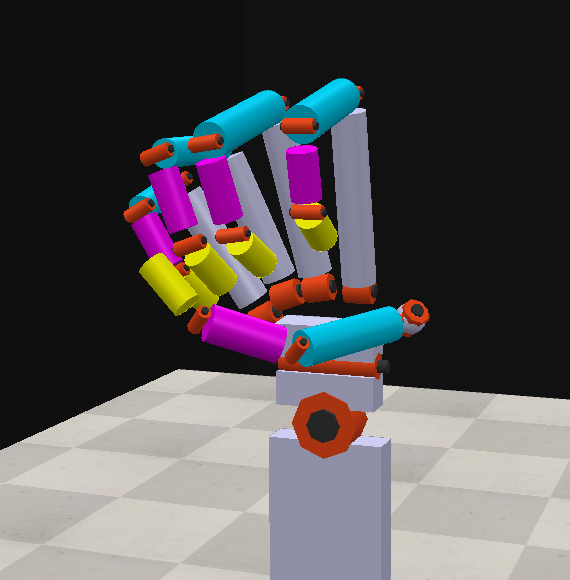
\includegraphics[width=\textwidth]{power_grip.png}
        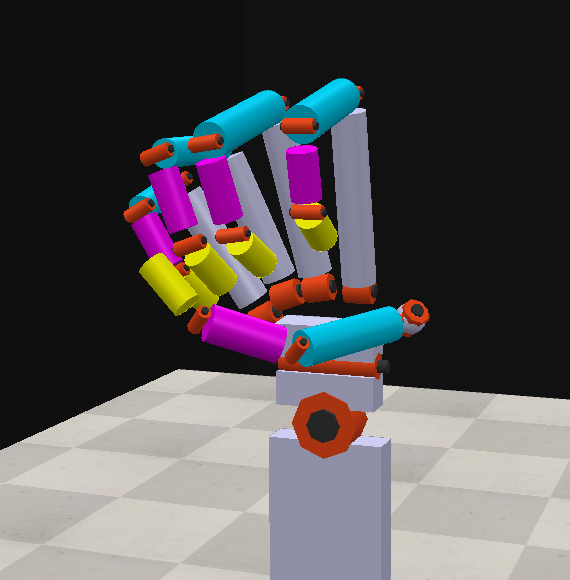
\includegraphics[height=8cm]{power_grip.png}
        \caption{Diagonal Volar grip (Power grip)}
    \end{subfigure}
    \caption{The four most used day-to-day poses, tested in a hand prosthetic simulation.}
    \label{fig:hand_pose_test}
\end{figure}


%TODO: Needs to be a figure of figures!
%\begin{figure}[h]
%\begin{center}
%\includegraphics[width=0.8\textwidth]{example-image-a}
%\caption{Example figure text}
%\end{center}
%\end{figure}

\subsection{Evaluation}

Based on a visual assessment of figure \ref{fig:hand_pose_test}, it can be concluded that the prosthetic hand is able to be posed similarly to the real-life reference.
The ROS2 interface created for the simulation allows for easy manipulation of the joint rotations, and because of this, achieving different poses becomes easy to do.
The hand simulation is able to achieve a wide range of motion because of its design and its ability to mimic the anatomy of the real hand.
From this it can be concluded that the prosthetic hand is proportionally correct and thus also allows for accurate posing, applicable in different day-to-day scenarios.

%\newpage
\subsection{Posing based on Network Output}

TODO: More here..

As a result of testing different network types and their applicability for creating suitable motor control output for a prosthetic hand, it would be ideal to test the network output on the prosthetic simulation.
For full video see appendix ??.
%TODO: Insert appendix here



%TODO: see Zhaolong2021 (page 10) for example of how to compare MSE for different neuron amounts, even for multiple subjects!



%TODO: Show graphs of different filters!
%TODO: Talk about what filters are and how they affect incoming signals, what type to use against what noise etc. 

\end{document}
